\documentclass[11pt]{article}
\usepackage[T1]{fontenc}
\usepackage[utf8]{inputenc}
\usepackage{lmodern}
\usepackage[a4paper,margin=25mm]{geometry}
\usepackage{amsmath,amssymb,amsthm,mathtools}
\usepackage{microtype,booktabs,array,graphicx,xcolor}
\usepackage{enumitem}
\usepackage[hyphens]{url}
\usepackage[colorlinks=true,linkcolor=blue!45!black,citecolor=blue!45!black,urlcolor=blue!50!black]{hyperref}
\usepackage{fancyhdr}
\hypersetup{pdftitle={Exact error correction for ramified branch measurements},pdfsubject={Total jets, contact trees, and optimal adversarial precision}}
\pagestyle{fancy}
\fancyhf{}
\fancyhead[L]{\small Ramified branch measurements}
\fancyhead[R]{\small Exact recovery and corruption}
\fancyfoot[C]{\thepage}
\setlength{\headheight}{14pt}
\setlength{\parskip}{4pt}
\setlength{\parindent}{0pt}
\setlist{itemsep=3pt,topsep=5pt}
\allowdisplaybreaks
\newtheorem{theorem}{Theorem}[section]
\newtheorem{lemma}[theorem]{Lemma}
\newtheorem{proposition}[theorem]{Proposition}
\newtheorem{corollary}[theorem]{Corollary}
\theoremstyle{definition}
\newtheorem{definition}[theorem]{Definition}
\newtheorem{remark}[theorem]{Remark}
\newcommand{\F}{\mathbf F}
\newcommand{\N}{\mathbf N}
\newcommand{\Z}{\mathbf Z}
\newcommand{\m}{\mathfrak m}
\newcommand{\ord}{\operatorname{ord}}
\newcommand{\supp}{\operatorname{supp}}
\newcommand{\Kern}{\mathcal K}
\newcommand{\E}{\mathcal E}
\newcommand{\Int}{\operatorname{Int}}
\newcommand{\capv}{\mathcal C}
\newcommand{\pos}[1]{\left(#1\right)_{+}}
\newcommand{\grhsha}{\texttt{72fead102f663d5c7a407964a13dc0cf9d977207}}
\newcommand{\pisha}{\texttt{4d7990202f9f106b2ffe8c209f073ad01d5e1987}}
\title{\textbf{Exact error correction for ramified branch measurements}\\[5pt]
\large Total jets, contact trees, and optimal adversarial precision}
\author{Research note with proofs and reproducible computations}
\date{26 November 2026}

\begin{document}
\maketitle
\thispagestyle{empty}
\begin{abstract}
We determine exactly how much of an arbitrary two-variable formal power series can be recovered from finitely truncated restrictions to clustered formal branches, even when some entire restrictions are erased or corrupted. The contact orders of the branches determine a greedy valuation sequence. We give the full observation kernel, the dimension of the unresolved target jet, and an exact relative block distance. The principal computational result is a scalar dynamic program that maximizes the number of retained branches compatible with a prescribed failure of recovery; it avoids enumerating all surviving subsets. For reduced Lubin--Tate branches, the inputs are explicit ramification depths. In a sharp binary example, sixteen branches determine all twenty-one coefficients of total degree at most five despite any three corrupted branch records if and only if fifteen coefficients are retained per branch. Fourteen coefficients admit an explicit ambiguity. A maximally packed survivor configuration fails to realize the worst adversary. We also give a closed formula for the precision at which the largest possible distance is reached. This extends the clean-data branch-recovery results in the specified ProveIt corpus. Bhargava's valuation orderings and Amini's fixed-tree factorial machinery are established ingredients; the proposed new contribution is the adversarial pruning optimization and its exact recovery consequences. Publication priority is not certified.
\end{abstract}

\section{The concrete result and its provenance}

Here is a precise result that requires no terminology from arithmetic geometry to state. A formal power series over $\F_2$ is a series whose coefficients are zero or one, with all arithmetic performed modulo two. No analytic convergence is involved.

\begin{theorem}[Sixteen binary branches]\label{thm:headline}
Let $H(X,Y)\in\F_2[[X,Y]]$ be arbitrary, and set
\[
 u_b(X)=(1+X)^b-1,\qquad b=0,1,\ldots,15.
\]
For each $b$, record the coefficients of degrees $0,\ldots,n-1$ of $H(X,u_b(X))$. Permit an adversary to replace any three of the sixteen records by arbitrary records of the same length. All twenty-one coefficients
\[
 [X^iY^j]H,\qquad i+j\le5,
\]
are uniquely determined for every $H$ and every such corruption if and only if $n\ge15$.
\end{theorem}

The unknown higher coefficients of $H$ are unrestricted. In particular, this is not the different interpolation problem in which $H$ is assumed to have total degree at most five. Section~\ref{sec:binary} proves the theorem and exhibits the indistinguishable records at $n=14$.

\subsection{What was extracted from the requested sources}

The upstream Lean development was inspected at commit
\begin{center}\small\grhsha.\end{center}
Its public interface proves RH and GRH for all Dirichlet characters of positive modulus, including imprimitive characters. The inspected statements do not assert a general Artin or automorphic GRH. The main construction compares upper and lower determinant bounds, combines short integral forms with a spanning argument, and obtains a one-sided prime-sum estimate. Its local ingredients include exact divisibility and sharpness questions for formal-series coefficients. These are the relevant methodological links to the present work \cite{sernau,guide,sharpness}.

The current Wikipedia page describes the announced formal proof. For the verification claim, we used the primary joint statement by the Lean FRO and Mathlib Initiative and Sutherland's verification record, which report statement matching and independent proof checks \cite{wiki,leanstatement,sutherland}. We did not rebuild the upstream development or replay its exported proof in this project.

The ProveIt snapshot is \pisha. Its scoped directory contains 61 unpacked earlier packets and 39 newer ZIP packets. Our screen covered the 61 delivery READMEs, six relevant mathematical \texttt{.tex} sections in full, and the text contents of seven selected newer ZIPs. The inventory and exact coverage are recorded in the accompanying provenance files. This is a focused comparison, not an independent validation of every claim in those packets.

The direct predecessor is the branch-recovery section of the packet on Lubin--Tate branches and graph towers, together with its earlier Lubin--Tate packet \cite{priorbranches,priorlt}. Those sources already give sharp precision for exactly $d$ clean branches, higher coefficient precision modulo powers of a uniformizer, optimal clean direction sets, and cancellation phenomena. We retain their formal-branch viewpoint and study redundant observations, arbitrary block corruptions, and the exact worst surviving configuration.

\subsection{Contribution and prior art}

The ingredients and proposed contribution should be distinguished precisely.
\begin{center}
\small
\begin{tabular}{@{}p{.43\linewidth}p{.51\linewidth}@{}}
\toprule
Ingredient & Status in this note\\
\midrule
Greedy valuation orderings and integral-valued polynomial bases & Established work of Bhargava; rederived in the finite case needed here \cite{bhargava97,bhargava09}.\\[4pt]
Factorials of a fixed weighted contact tree and merging child sequences & Established machinery of Amini \cite{amini}, especially Theorem 2.7.\\[4pt]
Qualitative finite recovery along reduced Lubin--Tate branches & Berger--Sprang, Lemma 4.2 \cite{bergersprang}.\\[4pt]
Sharp recovery from exactly $d$ clean branches & Present in the inspected ProveIt predecessors \cite{priorbranches,priorlt}.\\[4pt]
Maximizing retained leaves subject to failure of a target jet; exact block-error distance and sharp precision tradeoffs & Main extension developed and proved here.\\
\bottomrule
\end{tabular}
\end{center}

Classical $r$-removed orderings remove factors inside each greedy product; that is a different optimization \cite{johnson,krachun}. For example, with contacts $c(a,b)=2^{v_2(a-b)}$ on $\{0,1,2\}$, deleting one branch can retain $\{0,2\}$ with first nonzero factorial $2$. In contrast, the naturally shifted one-removed product after choosing $0,1$ has value $\min(c(2,0),c(2,1))=1$.

A targeted literature search did not locate the exact pruning-capacity recurrence or the corrupted-branch theorem below. This supports a proposed new extension relative to the sources inspected; it is not a guarantee of worldwide priority. The theorem is unconditional: it transfers local algebraic ideas and does not use RH as a hypothesis or claim to solve another general $L$-function conjecture.

\section{Branches, observations, and the target jet}\label{sec:setup}

Let $k$ be any field, $R=k[[X]]$, $A=k[[X,Y]]$, and $\m=(X,Y)$. Write $v=\ord_X$ on $R$, with $v(0)=+\infty$. Fix $N$ distinct branches
\[
 B=\{u_b:b\in I\}\subset XR,\qquad |I|=N.
\]
Their pairwise contacts are the positive integers
\begin{equation}\label{eq:contacts}
 s_{bc}=v(u_b-u_c),\quad b\ne c.
\end{equation}
They satisfy $s_{bc}\ge\min(s_{ba},s_{ac})$. For $n\ge0$, the observation map is
\[
 \E_n:A\longrightarrow (R/X^nR)^I,\qquad
 \E_n(H)_b=H(X,u_b(X))\bmod X^n.
\]
The substitution is well defined because $u_b\in XR$. Its $b$th coordinate is one \emph{block}, consisting of $n$ field coefficients. The target is
\[
 J_d(H)=H\bmod\m^d,\qquad 1\le d\le N.
\]
It comprises $d(d+1)/2$ coefficients. Recovery means that any two formal series consistent with the permitted observations have the same target jet. It does not mean recovery of their entire series.

\begin{definition}[Greedy valuation sequence]\label{def:greedy}
Order the branches $u_0,\ldots,u_{N-1}$ greedily: after choosing $u_0,\ldots,u_{j-1}$, choose an unused $u_j$ minimizing
\[
 \nu_j(B)=\sum_{i<j}v(u_j-u_i).
\]
The first branch is arbitrary and $\nu_0=0$. Put
\[
 P_j(Y)=\prod_{i<j}(Y-u_i),\qquad a_j=P_j(u_j),\qquad P_0=1.
\]
For any subset $S\subseteq B$, extend its sequence by $\nu_j(S)=+\infty$ for $j\ge |S|$, including $S=\varnothing$.
\end{definition}

The finite values of this sequence are independent of tie choices. We give a short proof, including the particular filtration facts required for total jets.

\section{The exact kernel and the amount of information recovered}\label{sec:kernel}

\begin{lemma}[Newton basis and intrinsicness]\label{lem:newton}
For $j<N$, the polynomials $P_i/a_i$, $0\le i\le j$, form an $R$-basis of the polynomials of degree at most $j$ in $k((X))[Y]$ that take values in $R$ on every branch of $B$. Consequently $\nu_j(B)$ is intrinsic. Moreover
\begin{equation}\label{eq:growth}
 \nu_{j+1}(B)\ge\nu_j(B)+1.
\end{equation}
\end{lemma}

\begin{proof}
At a previously chosen branch, $P_i$ vanishes. At every branch not yet chosen at step $i$, greediness gives $v(P_i(u_b))\ge v(a_i)=\nu_i$. Thus $P_i/a_i$ is integral valued on all $B$.

Every polynomial of degree at most $j$ has a unique expansion $\sum_{i=0}^j\alpha_iP_i/a_i$ over $k((X))$, by triangularity in the degree. If its values on $B$ are integral, successive evaluation at $u_0,u_1,\ldots,u_j$ shows $\alpha_i\in R$: higher terms vanish at $u_i$, its own normalized term equals one, and previously determined terms are integral. The converse follows from integral valuedness of the basis.

The possible coefficients of $Y^j$ therefore form exactly the fractional ideal $a_j^{-1}R$. That ideal is defined without a choice of ordering, so its valuation $-\nu_j$ is intrinsic. Finally, any candidate remaining at step $j+1$ had cost at least $\nu_j$ at step $j$, and has acquired one additional contact of at least one with $u_j$. This proves~\eqref{eq:growth}.
\end{proof}

\begin{lemma}[Division and total-degree filtration]\label{lem:division}
Every $H\in A$ has a unique expansion
\begin{equation}\label{eq:division}
 H=P_NQ+\sum_{j=0}^{N-1}c_j(X)P_j(Y),\qquad Q\in A,\quad c_j\in R.
\end{equation}
For a nonzero remainder in this expansion,
\begin{equation}\label{eq:order}
 \ord_{\m}\!\left(\sum_{j<N}c_jP_j\right)
 =\min_{j<N}\bigl(v(c_j)+j\bigr).
\end{equation}
Since $P_N\in\m^N$, $H$ and its remainder have the same target jet for $d\le N$.
\end{lemma}

\begin{proof}
For $u\in XR$, the difference $H(X,Y)-H(X,u)$ is divisible in $A$ by $Y-u$. This follows term by term from
\[
 Y^a-u^a=(Y-u)\sum_{h=0}^{a-1}Y^{a-1-h}u^h;
\]
the resulting series converges formally in the $(X,Y)$-adic topology. Apply this division successively at $u_0,\ldots,u_{N-1}$. It gives~\eqref{eq:division}. Successive evaluation of a putative zero remainder at the same branches forces each coefficient $c_j$ to vanish, because $a_j\ne0$ in the domain $R$. The quotient is then unique as well.

The coefficient of $Y^i$ in $P_j$, for $i<j$, is divisible by $X^{j-i}$, and $P_j$ is monic of $Y$-degree $j$. Each summand has total order $v(c_j)+j$. At the smallest such order, choose the largest $j$ attaining the minimum. Its leading homogeneous term has a nonzero coefficient at $X^{v(c_j)}Y^j$ that terms with smaller $Y$-degree cannot cancel. Terms with larger $j$ have strictly greater total order. This proves~\eqref{eq:order}.
\end{proof}

\begin{theorem}[Exact observation kernel]\label{thm:kernel}
Let $\Kern_n(B)=\ker\E_n$. Then
\begin{equation}\label{eq:kernel}
 \boxed{\displaystyle
 \Kern_n(B)=P_NA+
 \bigoplus_{j=0}^{N-1}X^{\max(0,n-\nu_j(B))}R P_j.}
\end{equation}
The direct sum refers to the space of remainders in~\eqref{eq:division}.
\end{theorem}

\begin{proof}
The multiple of $P_N$ vanishes on every branch. For the remainder $R_H=\sum c_jP_j$, its observations vanish modulo $X^n$ exactly when $X^{-n}R_H$ is integral valued on $B$. By Lemma~\ref{lem:newton}, this is equivalent to $X^{-n}c_ja_j\in R$ for every $j$, or $v(c_j)\ge n-\nu_j$. We already have $c_j\in R$, giving $v(c_j)\ge\max(0,n-\nu_j)$. This is both necessary and sufficient.
\end{proof}

\begin{corollary}[Complete recovery and unresolved dimension]\label{cor:jet}
The target $J_d(H)$ is determined by the clean observations if and only if
\begin{equation}\label{eq:clean}
 \boxed{n\ge\nu_{d-1}(B)+1.}
\end{equation}
More precisely, the greatest completely recoverable total-jet order is
\begin{equation}\label{eq:D}
 D_n(B)=\#\{j<N:\nu_j(B)<n\}.
\end{equation}
For $d\le N$, the dimension of the unresolved subspace of the target is
\begin{equation}\label{eq:ambiguity}
 \dim_k\frac{\Kern_n(B)+\m^d}{\m^d}
 =\sum_{j=0}^{d-1}
 \max\bigl(0,d-j-\max(0,n-\nu_j(B))\bigr).
\end{equation}
\end{corollary}

\begin{proof}
Suppose $n\ge\nu_{d-1}+1$. For $j<d$, equation~\eqref{eq:growth} gives
\[
 n-\nu_j+j\ge\nu_{d-1}+1-\nu_j+j\ge d.
\]
All kernel terms with $j\ge d$ already have total order at least $d$. The kernel is therefore contained in $\m^d$.

Conversely, $P_{d-1}$ has total order exactly $d-1$ and takes values of order at least $\nu_{d-1}$ on every branch. Hence, if $n\le\nu_{d-1}$, the series $0$ and $P_{d-1}$ have identical observations and different target jets. If one asks for a jet beyond order $N$, the exact kernel element $P_N$ prevents recovery. These facts prove~\eqref{eq:D}.

The residue classes $X^iP_j$ with $i+j<d$ form a basis of $A/\m^d$, by the triangular filtration argument. In the $j$th Newton component the kernel contains exactly the powers with $i\ge\max(0,n-\nu_j)$. Counting those with $i+j<d$ gives~\eqref{eq:ambiguity}.
\end{proof}

If fewer than $d$ branches survive, recovery of $J_d$ is impossible at any precision: their full branch product is a nonzero element of total order below $d$ that vanishes on all of them. This explains the $+\infty$ convention for missing factorials.

\section{An exact distance for different target jets}\label{sec:distance}

For vectors of observations, count a coordinate as different if any of the $n$ coefficients in that block differs. Define the relative distance
\begin{equation}\label{eq:distance-def}
 \delta_d(n;B)=
 \min_{H\notin\m^d}\#\{b:\E_n(H)_b\ne0\}.
\end{equation}
It is the minimum distance between observations belonging to two different target jets, allowing arbitrary higher terms in both series. The distance can be zero. It is not necessarily the minimum distance of the entire image code, since nonzero words arising from $H\in\m^d$ do not change the desired output.

\begin{definition}[Adversarial retention capacity]\label{def:capacity}
For $r\ge0$ and integer $T$, put
\[
 \capv_B(r,T)=
 \max\{|S|:S\subseteq B,\ \nu_r(S)\ge T\}.
\]
The empty set is permitted, and missing factorials are $+\infty$. Thus $\capv_B$ is defined at every indicated argument.
\end{definition}

\begin{theorem}[Distance and correction criterion]\label{thm:distance}
For $1\le d\le N$ and $n\ge0$,
\begin{equation}\label{eq:distance}
 \boxed{\delta_d(n;B)=N-\capv_B(d-1,n).}
\end{equation}
For nonnegative integers $t,e$, recovery of $J_d(H)$ for every $H$, despite at most $t$ arbitrarily corrupted blocks and at most $e$ flagged erased blocks, is possible if and only if
\begin{equation}\label{eq:correct}
 \boxed{2t+e<\delta_d(n;B).}
\end{equation}
All failure statements admit explicit witnesses built from branch products.
\end{theorem}

\begin{proof}
For a set $S$ of at least $d$ branches, Corollary~\ref{cor:jet} says that some $H\notin\m^d$ can vanish modulo $X^n$ on all $S$ exactly when $\nu_{d-1}(S)\ge n$. If $|S|<d$, the product $\prod_{u\in S}(Y-u)$ is such an $H$ at every precision. Thus the largest possible set of zero blocks of a series with a nonzero target is exactly $\capv_B(d-1,n)$. This proves~\eqref{eq:distance}. The minimum is attained: use $P_{d-1}$ on a maximizing $S$ if $|S|\ge d$, and its full branch product otherwise. Any additional zero blocks would contradict maximality of $|S|$.

For sufficiency in~\eqref{eq:correct}, two explanations of the same received data can differ only on the union of their two error sets and the erased positions, a set of size at most $2t+e$. Different target jets would contradict the distance bound.

For necessity, take two true words with different target jets at distance $\delta_d$. If $\delta_d=0$, they are already indistinguishable. Otherwise, erase up to $e$ differing coordinates so that at most $2t$ differences remain; split the remaining differences into two groups, each of size at most $t$. Choose a received word that follows the first true word on one group and the second on the other. It lies within the permitted error budget of each explanation. This proves impossibility and gives a construction.
\end{proof}

For a fixed known erasure set $E$, apply the theorem directly to $B\setminus E$. Equation~\eqref{eq:correct} with $e$ is the uniform guarantee over all choices of at most $e$ erasures. In particular, no finite precision can give that uniform guarantee when $N-e-2t<d$.

\subsection{A finite decoder}

Whenever recovery is possible, $n\ge d$. Because every $u_b\in XR$, terms of total degree at least $n$ make no contribution modulo $X^n$. One may therefore use the $n(n+1)/2$ coefficients of total degree below $n$ as finite unknowns. Enumerate the possible erroneous block sets, discard those equations, and solve the remaining linear systems over $k$. Every consistent solution has the same degree-$<d$ jet under~\eqref{eq:correct}. The actual error set supplies at least one solution.

This proves constructive recoverability over an effective field, but makes no claim of a fast general error-location algorithm. The supplied binary reference decoder uses this procedure and first checks the exact distance condition. That guard is necessary: choosing zero for free variables without checking uniqueness can conceal unresolved jets.

\section{The adversarial capacity is computable by a scalar tree recursion}\label{sec:dp}

The contacts in~\eqref{eq:contacts} determine a finite rooted tree. Its leaves are the branches. For $N=1$, use a single leaf; assume $N\ge2$ in the following construction. The root has an incoming stem of length $\min_{b\ne c}s_{bc}$. At any cluster, partition its leaves by the relation $s_{bc}$ strictly greater than that cluster's minimum contact; these equivalence classes are its children. Repeat until singletons. The incoming length $\ell_v$ of an internal node is its contact level minus the parent's contact level. Leaf edges may have length zero. The common path length of two distinct leaves equals their contact.

At a node $v$, use only the residual common path below its parent. For a selected set of its descendant leaves, write $\lambda_j^v(S)$ for its greedy sequence in that residual tree. Missing entries are $+\infty$. At the root this is $\nu_j(S)$.

\begin{lemma}[Fixed-tree merge]\label{lem:merge}
Let $v$ be an internal node, with children $c$. Let $z_0\le z_1\le\cdots$ be the sorted union of the finite sequences $\lambda_i^c(S\cap B_c)$. Then
\begin{equation}\label{eq:merge}
 \lambda_j^v(S)=j\ell_v+z_j,\qquad 0\le j<|S|.
\end{equation}
All these sequences are nondecreasing and independent of greedy tie choices.
\end{lemma}

\begin{proof}
A candidate selected after $j$ total choices pays $j\ell_v$ for the common incoming segment. If $i$ prior choices were in its child, it pays that child's next greedy cost in addition. The first term is the same for every candidate. By induction up from leaves, each child offers a nondecreasing stream of costs; choosing the smallest available next cost merges the streams. Adding $j\ell_v$ preserves monotonicity and proves the formula. This is the finite form of the established tree-factorial mechanism \cite{amini}.
\end{proof}

Define
\[
 \capv_v(r,T)=\max\{|S|:S\subseteq B_v,\ \lambda_r^v(S)\ge T\},
 \qquad N_v=|B_v|.
\]

\begin{theorem}[Scalar adversarial pruning recursion]\label{thm:dp}
If $T\le0$ or $r\ge N_v$, then $\capv_v(r,T)=N_v$. At a singleton leaf and $T>0$,
\[
 \capv_v(0,T)=0,\qquad \capv_v(r,T)=1\quad(r\ge1).
\]
At an internal node,
\begin{equation}\label{eq:dp}
 \boxed{\displaystyle
 \capv_v(r,T)=
 \max_{\substack{r_c\in\N\ (c\text{ a child})\\\sum_c r_c\le r}}
 \sum_c\capv_c(r_c,T-r\ell_v).}
\end{equation}
The recurrence is exact and a maximizing leaf set can be recovered by backtracking maximizing allocations.
\end{theorem}

\begin{proof}
Put $U=T-r\ell_v$. Formula~\eqref{eq:merge}, including the infinite tail, gives
\[
 \lambda_r^v(S)\ge T
 \quad\Longleftrightarrow\quad z_r\ge U.
\]
The latter says that at most $r$ entries in the combined child streams are \emph{strictly} less than $U$. If $h_c$ is the number of such entries in child $c$, it is equivalent to $\sum_c h_c\le r$. The constraint $h_c\le r_c$ is exactly $\lambda_{r_c}^c(S\cap B_c)\ge U$.

Every admissible $S$ therefore yields an allocation $r_c=h_c$ in the right side of~\eqref{eq:dp}, and its cardinality is at most that side. Conversely, for any allowed allocation, choose a maximizing child set for each term. Their disjoint union has at most $r$ entries below $U$, so is admissible at $v$, and its cardinality is the sum in the formula. Both inequalities and the backtracking assertion follow. The base cases follow directly from nonnegative costs and the sequence $[0]$ of a singleton.
\end{proof}

The outer maximization here changes the set of leaves retained. Lemma~\ref{lem:merge} alone computes the sequence on a fixed set; it does not optimize this outer problem. Keeping only one ``most clustered'' survivor set is insufficient, as Section~\ref{sec:binary} demonstrates.

\subsection{Complexity and precision boundaries}

For a query with $r\le d-1$, use ranks $0,\ldots,d-1$ and thresholds $1,\ldots,T_{\max}$. Nonpositive thresholds use a base case. Combining child tables is a max convolution in the rank budget. On a compact tree with $O(N)$ nodes, a straightforward table costs $O(Nd^2T_{\max})$ arithmetic operations. This is pseudopolynomial in numeric precision, not a strongly polynomial bound in the bit length of the contact orders.

For $d\le N$, a sufficient saturation bound is $T_{\max}=1+(d-1)s_{\max}$, where $s_{\max}$ is the largest pairwise contact; take $s_{\max}=0$ when $N=1$. The exact saturation value is given next. On a full Lubin--Tate grid of $N=q^L$ branches with $L\ge1$, $s_{\max}=N/q$, so the full relevant precision table is polynomial in $N$ for fixed $q,d$. Isomorphic subtrees can share tables. None of these bounds refers to the separate cost of locating corrupted blocks.

\section{A closed formula for reaching the largest possible distance}\label{sec:saturation}

\begin{theorem}[Exact saturation precision]\label{thm:saturation}
Always $\delta_d(n;B)\le N-d+1$. Let $r=d-1$, and for each $b$ sum the $r$ largest contacts $s_{bc}$ with other branches. Then the least precision attaining $N-d+1$ is
\begin{equation}\label{eq:saturation}
 \boxed{\displaystyle n_{\mathrm{sat}}=
 1+\max_b\left(\text{sum of the $d-1$ largest contacts from $b$}\right).}
\end{equation}
The empty sum for $d=1$ is zero.
\end{theorem}

\begin{proof}
The product of any $d-1$ branch equations has total order $d-1$ and vanishes on those branches. It proves the distance upper bound. By~\eqref{eq:distance}, equality occurs exactly when no series with a nonzero target jet can vanish modulo $X^n$ on any $d$-element subset.

For a $d$-element set $S$, put $\Delta_b=\prod_{c\in S\setminus\{b\}}(u_b-u_c)$. Lagrange interpolation over $k((X))$ shows that the leading coefficients of degree-at-most-$d-1$ polynomials integral valued on $S$ form the ideal generated by $\Delta_b^{-1}$, $b\in S$. Values at the $d$ points may be assigned arbitrarily in $R$, so this is an equality of ideals. Its valuation is $-\max_b v(\Delta_b)$. Lemma~\ref{lem:newton} identifies the same ideal with $a_{d-1}^{-1}R$. Hence
\begin{equation}\label{eq:lastfactorial}
 \nu_{d-1}(S)=\max_{b\in S}\sum_{c\in S\setminus\{b\}}s_{bc}.
\end{equation}
All $d$-subsets recover exactly when $n$ exceeds their largest such factorial. For fixed $b$, maximize the row sum by retaining its $d-1$ highest-contact neighbors. This is precisely~\eqref{eq:saturation}.
\end{proof}

The saturation formula has a simple nearest-neighbor form. The precision for an intermediate error budget usually needs the full capacity recursion; substituting the saturation expression into every smaller error budget would be wrong.

\section{Reduced Lubin--Tate branches}\label{sec:LT}

Let $\mathcal O$ be the ring of integers of a finite extension of $\mathbf Q_p$, with uniformizer $\pi$, residue field $k$ of cardinality $q$, and $v_\pi(\pi)=1$. For a Lubin--Tate formal $\mathcal O$-module, set
\[
 u_b(X)=[b](X)\bmod\pi,\qquad b\in\mathcal O.
\]
These branches have contacts
\begin{equation}\label{eq:LTcontact}
 v_X(u_b-u_c)=q^{v_\pi(b-c)}\quad(b\ne c).
\end{equation}
Indeed, the formal group law makes $[b]-[c]$ a unit multiple of $[b-c]$. If $b-c=\pi^ha$ with $a$ a unit, then $[a]$ has invertible linear coefficient, while $[\pi](X)\equiv X^q\pmod\pi$. Iteration gives the asserted first nonzero degree. This also proves distinctness of the reduced branches. The general recovery and capacity results therefore apply using ramification depths alone.

For $L\ge1$, take one representative of each class modulo $\pi^L$. The tree has $q$ children at each level. The root stem has length $1$, and an internal node of depth $h\ge1$ has incoming increment
\[
 \ell_h=q^h-q^{h-1}=(q-1)q^{h-1}.
\]
There are $q^L$ singleton leaves. No coefficients of the formal group law need to be computed to evaluate the exact distance.

\begin{corollary}[Full-grid saturation]\label{cor:grid}
For this full residue grid, $N=q^L$, $1\le d\le N$, and $r=d-1$,
\begin{equation}\label{eq:gridsat}
 \boxed{\displaystyle n_{\mathrm{sat}}
 =1+r+\sum_{h=1}^{L-1}(q^h-q^{h-1})\min(r,q^{L-h}-1).}
\end{equation}
\end{corollary}

\begin{proof}
Every one of the $r$ selected neighbors contributes the baseline contact $1$. For each $h\ge1$, exactly $q^{L-h}-1$ other grid points are congruent to a fixed branch modulo $\pi^h$. The $r$ closest neighbors include $\min(r,q^{L-h}-1)$ of them, because these balls are nested. Each contributes the increment $q^h-q^{h-1}$. Summing the increments and applying Theorem~\ref{thm:saturation} proves the formula.
\end{proof}

These results concern coefficients over the residue field $k$. They do not assert the same contact-only formulas over $\mathcal O/\pi^a$ for $a>1$, where additional cancellation can occur. The predecessor packets analyze such clean-data cancellations; their extension to adversarial records is a separate problem.

\section{The sharp binary example}\label{sec:binary}

Take the multiplicative formal group over $\Z_2$. Its reductions are
\[
 u_b=(1+X)^b-1\in\F_2[X],\qquad 0\le b<16,
\]
and $s_{bc}=2^{v_2(b-c)}$. The contact tree has incoming increments $1,1,2,4$ above singleton leaves. The target order is $d=6$, so the rank budget in the capacity recurrence is $r=5$.

\subsection{An exact upper certificate}

The two parity subtrees each contain eight leaves and have identical residual geometry. At root threshold $n=14$, the child threshold is $14-5=9$; at $n=15$ it is $10$. Applying~\eqref{eq:dp} inside either parity subtree gives
\begin{center}
\begin{tabular}{@{}lrrrrrr@{}}
\toprule
Child rank budget $r_c$ & 0&1&2&3&4&5\\
\midrule
$\capv_c(r_c,9)$ &0&1&4&6&8&8\\
$\capv_c(r_c,10)$&0&1&4&5&8&8\\
\bottomrule
\end{tabular}
\end{center}
The root splits its budget as $a+(5-a)$. The resulting sums are
\[
\begin{array}{c|rrrrrr}
 a&0&1&2&3&4&5\\ \hline
 n=14&8&9&10&10&9&8\\
 n=15&8&9&9&9&9&8
\end{array}
\]
and hence
\begin{equation}\label{eq:binarydistance}
 \capv_B(5,14)=10,\quad \capv_B(5,15)=9,
 \qquad \delta_6(14;B)=6,\quad\delta_6(15;B)=7.
\end{equation}
The strict condition $2t<\delta$ gives impossibility at $n=14$ and sufficiency at $n=15$ for $t=3$. Monotonicity in precision proves Theorem~\ref{thm:headline} for all $n$.

For completeness, the small child table can be verified without a program. A two-leaf subtree below a four-leaf node has residual spectrum $[0,4]$. For the four-leaf node, whose incoming increment is $2$, maximal capacities at positive $U$ are
\[
\begin{aligned}
 C_0(U)&=0,\\
 C_1(U)&=\begin{cases}4&U\le2,\\2&3\le U\le6,\\1&U\ge7,\end{cases}\\
 C_2(U)&=\begin{cases}4&U\le8,\\2&U\ge9,\end{cases}\qquad
 C_3(U)=\begin{cases}4&U\le10,\\3&U\ge11,\end{cases}
\end{aligned}
\]
and $C_r(U)=4$ for $r\ge4$. These follow from the possible selected-set spectra: a same-child pair has $[0,6]$, a split pair $[0,2]$, any three leaves $[0,2,8]$, and all four $[0,2,8,10]$. At the eight-leaf parity node, use child threshold $U=T-r_c$ and maximize $C_a(U)+C_{r_c-a}(U)$. This produces every entry of the displayed table.

\subsection{Why the most packed survivors are not worst}

A natural packed ten-element survivor set is
\[
 S_P=\{0,2,4,6,8,10,12,14,1,9\}.
\]
It retains all eight even directions and a closely paired pair of odd directions. Its greedy sequence is
\[
 (0,1,3,7,9,12,18,20,24,26).
\]
Its target-$6$ clean cutoff is $12+1=13$. But the less concentrated set
\[
 S_A=\{0,1,2,4,5,8,9,10,12,13\}
\]
has sequence
\[
 (0,1,3,6,8,14,16,19,21,24),
\]
so its target-$6$ cutoff is $14+1=15$. The two spectra cross. One configuration cannot be declared the worst for every target order simply from its visual clustering.

\begin{figure}[!ht]
\centering
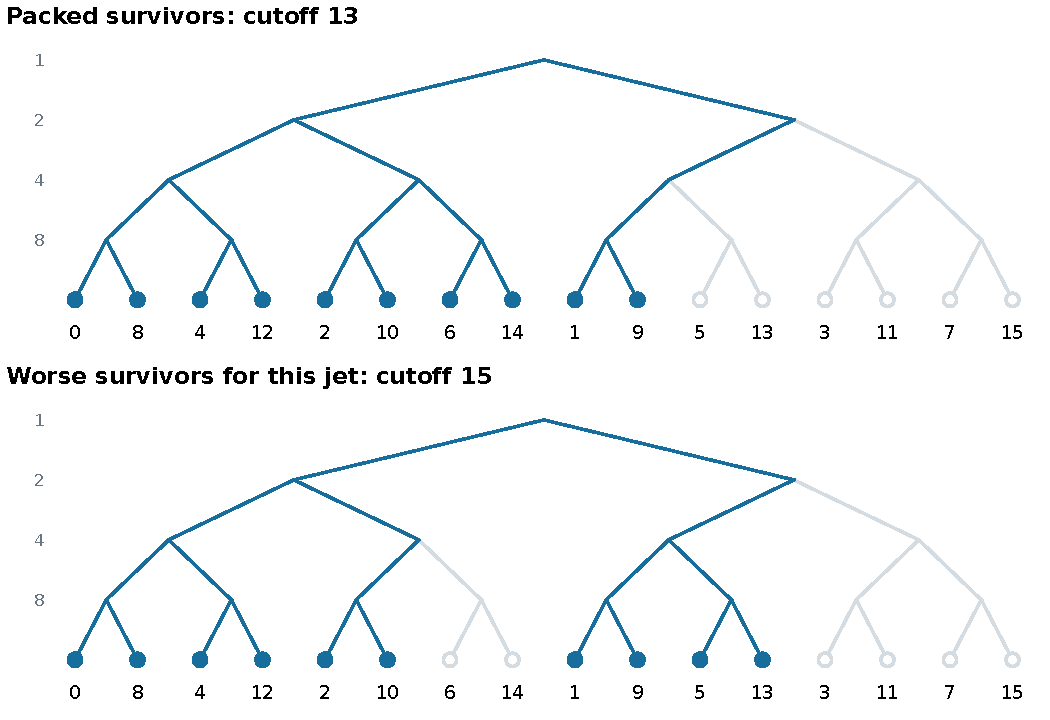
\includegraphics[width=.95\linewidth]{figures/survivor_trees.pdf}
\caption{Two ten-branch survivor sets inside the same sixteen-branch contact tree. Filled leaves survive; empty leaves are removed. Labels are ordered by low-order binary digits. Numbers at the left are cumulative contacts at each branching level. The more packed pattern has a smaller sixth factorial.}
\label{fig:trees}
\end{figure}

\subsection{An explicit indistinguishable pair}

A greedy ordering of $S_A$ begins $0,1,2,5,4,10$. Set
\begin{equation}\label{eq:witness}
 H_*(X,Y)=\prod_{b\in\{0,1,2,4,5\}}(Y-u_b(X)).
\end{equation}
Its degree-five homogeneous part is
\[
 Y^3(Y-X)^2=Y^5+X^2Y^3\ne0\quad\text{over }\F_2.
\]
At $n=14$, it vanishes on exactly the ten branches $S_A$. The six other branches are
\[
 D=\{3,6,7,11,14,15\},
\]
where its orders are respectively $7,10,7,7,10,7$, all below $14$.

Let a received record equal $H_*(X,u_b)\bmod X^{14}$ at $b=3,6,7$ and equal zero elsewhere. It differs from the zero-series record at three blocks. It differs from the $H_*$ record at the other three blocks $11,14,15$. Thus the same received data admit two explanations with different target jets and only three corruptions each. This proves the lower bound by an actual series, not just a cardinality argument. Erasing any two of the six positions similarly gives a two-error, two-erasure ambiguity.

\subsection{The complete precision--distance tradeoff}

The same recurrence gives the entire relative-distance diagram.
\begin{center}
\begin{tabular}{@{}lrrl@{}}
\toprule
Retained coefficients $n$ & $\capv_B(5,n)$ & $\delta_6(n;B)$ & Errors correctable, $e=0$\\
\midrule
$0$--$9$ &16&0&Even clean recovery fails\\
$10$ &12&4&1\\
$11$--$14$ &10&6&2\\
$15$--$17$ &9&7&3\\
$18$ &8&8&3\\
$19$--$20$ &6&10&4\\
$n\ge21$ &5&11&5\\
\bottomrule
\end{tabular}
\end{center}
For erasures as well, replace the last column by the exact condition $2t+e<\delta_6(n;B)$. At $n=15$, for example, the budgets $(t,e)=(3,0),(2,2),(1,4),(0,6)$ all work.

\begin{figure}[!ht]
\centering
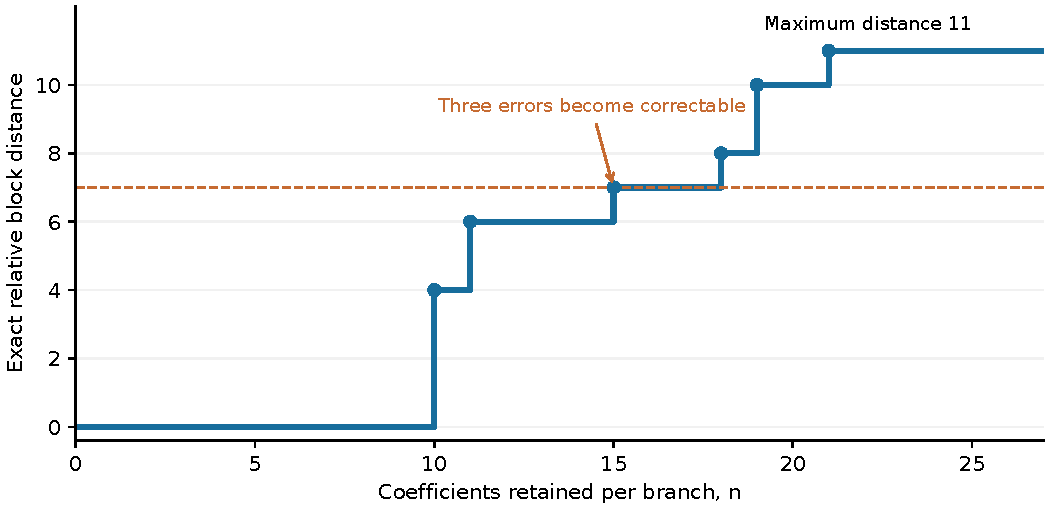
\includegraphics[width=.95\linewidth]{figures/precision_distance.pdf}
\caption{Exact distance for the target of twenty-one coefficients on the sixteen binary branches. The steps are computed by the proved capacity recurrence. Distance seven is the threshold for three arbitrary block errors.}
\label{fig:distance}
\end{figure}

Corollary~\ref{cor:grid} gives the saturation point directly:
\[
 n_{\mathrm{sat}}=1+5+1\cdot5+2\cdot3+4\cdot1=21.
\]
The maximal distance is $16-6+1=11$. Equation~\eqref{eq:ambiguity} also shows that the clean sixteen-branch data leave a two-dimensional target ambiguity at $n=9$ and none at $n=10$. For $S_A$, the ambiguity at $n=14$ is exactly one-dimensional.

\begin{corollary}[An infinite sharp family]\label{cor:scaled}
Replace the directions $b=0,\ldots,15$ by $2^ab$ for any integer $a\ge0$. The exact precision for recovering the same degree-$<6$ target with any three corrupted blocks is
\[
 n=14\cdot2^a+1.
\]
Clean recovery on the packed ten-element pattern needs only $12\cdot2^a+1$, and saturation of the full sixteen-branch distance occurs at $20\cdot2^a+1$.
\end{corollary}

\begin{proof}
All contacts are multiplied by $2^a$, since $u_{2^ab}(X)=u_b(X^{2^a})$ over $\F_2$. Every greedy factorial of every survivor subset is therefore multiplied by that factor. Apply the strict inequalities in the clean-recovery and distance theorems. The target remains the total-degree-$<6$ jet in the original variables.
\end{proof}

\section{Verification, reproducibility, and formalization status}\label{sec:checks}

The proofs above are mathematical proofs. The finite computations provide independent checks and exact certificates for the example; they do not replace those proofs.

The package contains a Python implementation using only the standard library for all verification and decoding. It performs the following checks:
\begin{itemize}
\item compares direct greedy sequences with tree merging on all 256 subsets of an eight-branch grid;
\item compares 240 capacity states with independent exhaustive subset calculations, including backtracked witnesses;
\item examines all $\binom{16}{10}=8008$ ten-branch survivor sets, finding maximum sixth factorial exactly $14$;
\item checks selected thresholds by direct substitution matrices over $\F_2$, retaining unknown higher terms up to the observation cutoff;
\item evaluates the explicit ambiguity series and its six nonzero blocks at precision $14$;
\item decodes a deterministic example with three corrupted records at precision $15$, inspecting all $\binom{16}{3}=560$ candidate error-location sets;
\item rejects an uncertified decoding case where free variables would otherwise conceal a second target jet.
\end{itemize}

A separate internal derivation and implementation also checked direct substitution over $\F_2,\F_3,\F_5$, tie independence, and random contact trees. This is internal adversarial review, not external peer review. The provided core reproduction requires:
\begin{verbatim}
python3 code/verify.py
python3 code/make_figures.py     # optional; requires matplotlib
pdflatex paper.tex
pdflatex paper.tex
\end{verbatim}
The exact JSON and CSV outputs are included. Figures are provided in vector PDF and PNG formats.

No Lean proof of the new theorem was compiled in this project. The included formalization plan separates the finite tree theorem, valuation/Newton-basis algebra, the total-jet filtration, and the coding-distance argument. A complete formalization would need to connect these layers; the upstream GRH proof is not imported by this result.

\section{What the result adds, and the remaining boundary}

The output of the method is a sharp answer to a finite information problem: given a contact tree, a truncation length, and a target total jet, it computes exactly how many entire measurements may be lost or falsified. It also constructs a matching ambiguity when a proposed budget is too large. The key new optimization runs over all retained subsets and remains sensitive to the target order; the crossing survivor spectra show why a simple geometric packing rule does not solve it.

Several extensions remain open within this note: efficient error-location algorithms beyond subset enumeration; exact formulas for unequal truncation lengths; and adversarial recovery over $\mathcal O/\pi^a$ with $a>1$. None is needed for the stated theorem. The result provides a completed local extension of the specified research corpus, with a transparent boundary between classical machinery, newly derived consequences, and unproved future directions.

\begin{thebibliography}{99}
\small\raggedright
\bibitem{sernau} L. Sernau and collaborators, \emph{GRH for Dirichlet $L$-functions, in Lean 4}, 2026. Commit \grhsha. \url{https://github.com/lsernau/grh-lean}. Public statements: \texttt{grh/src/Statements.lean}; proofs: \texttt{grh/src/Main.lean}.
\bibitem{guide} Same repository, \emph{Reading guide}, at the pinned commit. \href{https://github.com/lsernau/grh-lean/blob/72fead102f663d5c7a407964a13dc0cf9d977207/grh/GUIDE.md}{\texttt{grh/GUIDE.md}}. Also \path{New/Reduction/MainInequality.lean} and \path{New/Reduction/Lattices/TwistedLattice.lean}.
\bibitem{sharpness} Same repository, \href{https://github.com/lsernau/grh-lean/blob/72fead102f663d5c7a407964a13dc0cf9d977207/grh/src/New/Derivatives/Sharpness/BoundAttained.lean}{\emph{Sharpness of the valuation bound}}, \path{New/Derivatives/Sharpness/BoundAttained.lean}.
\bibitem{wiki} Wikipedia contributors, \emph{Riemann hypothesis}, inspected 26 November 2026. \url{https://en.wikipedia.org/wiki/Riemann_hypothesis}. Used for the requested contextual comparison; the verification claim was checked against primary records.
\bibitem{leanstatement} Lean FRO and Mathlib Initiative, \emph{Lean verification of the Riemann Hypothesis}, joint statement, 21 November 2026. \url{https://leanprover-community.github.io/blog/posts/riemann-hypothesis/}.
\bibitem{sutherland} A. Sutherland, \emph{Verification files for the Lean proof of the Riemann Hypothesis}, MIT, updated 25 November 2026. \url{https://math.mit.edu/~drew/grh/}.
\bibitem{priorbranches} ProveIt research packet, \emph{Sharp local bounds from methods in the Lean proof of Dirichlet GRH}, section \emph{How much of each formal branch must one observe?}, 2026. Snapshot \pisha. \href{https://github.com/VladimirReshetnikov/ProveIt/blob/4d7990202f9f106b2ffe8c209f073ad01d5e1987/Analysis/GeneralizedRiemannHypothesis/Research/grh_transfers_lubin_tate_and_graph_towers/branches.tex}{Branch-recovery source, \texttt{branches.tex}}. Git blob \texttt{50b914abc1d738fdeae53dd39296254461c6279a}.
\bibitem{priorlt} ProveIt research packet, \emph{Optimal signings of square cycles and sharp Lubin--Tate jet recovery}, 2026. Same snapshot. \href{https://github.com/VladimirReshetnikov/ProveIt/blob/4d7990202f9f106b2ffe8c209f073ad01d5e1987/Analysis/GeneralizedRiemannHypothesis/Research/grh_transfers_cycle_signings_and_lubin_tate/lubin_tate.tex}{Lubin--Tate source, \texttt{lubin\_tate.tex}}. Git blob \texttt{93fcf9cf65cfcd2208a1c32eb7e478a365569597}.
\bibitem{bhargava97} M. Bhargava, \emph{$P$-orderings and polynomial functions on arbitrary subsets of Dedekind rings}, J. Reine Angew. Math. \textbf{490} (1997), 101--127. \url{https://doi.org/10.1515/crll.1997.490.101}.
\bibitem{bhargava09} M. Bhargava, \emph{On $P$-orderings, rings of integer-valued polynomials, and ultrametric analysis}, J. Amer. Math. Soc. \textbf{22} (2009), 963--993. \url{https://doi.org/10.1090/S0894-0347-09-00638-9}.
\bibitem{amini} O. Amini, \emph{Logarithmic tree factorials}, arXiv:1611.02142, 2016; author draft February 2017. \url{https://arxiv.org/abs/1611.02142}. Author text: \url{https://www.math.ens.psl.eu/~amini/Publications/TreeFactorials.pdf}.
\bibitem{bergersprang} L. Berger and J. Sprang, \emph{Integer-valued polynomials and $p$-adic Fourier theory}, arXiv:2502.18053v2, 2025, especially Lemmas 4.1--4.2. \url{https://arxiv.org/abs/2502.18053}.
\bibitem{johnson} K. Johnson, \emph{Computing $r$-removed $P$-orderings and $P$-orderings of order $h$}, Actes des rencontres du CIRM \textbf{2} (2010), no. 2, 33--40. \url{https://doi.org/10.5802/acirm.31}.
\bibitem{krachun} D. Krachun and R. Mirgalimova, \emph{Strong greedoid structure of $r$-removed $P$-orderings}, Electronic J. Combin. \textbf{31} (2024), no. 4, P4.40. \url{https://doi.org/10.37236/12403}.
\end{thebibliography}
\end{document}
